\documentclass[11pt,a4paper]{article}
\usepackage[margin=2.2cm]{geometry}
\usepackage[T1]{fontenc}
\usepackage{lmodern,microtype}
\usepackage{graphicx,booktabs,tabularx,float,caption,xcolor,enumitem,amsmath,array,multirow}
\usepackage[hidelinks]{hyperref}
\graphicspath{{../figures/}{../../results/plots/}}
\captionsetup{font=small,labelfont=bf}
\setlist{itemsep=2pt,topsep=4pt}
\newcolumntype{R}{>{\raggedleft\arraybackslash}X}
\makeatletter % float-only pages: stack floats from the top instead of spreading them out
\setlength{\@fptop}{0pt}\setlength{\@fpsep}{14pt}\setlength{\@fpbot}{0pt plus 1fil}
\makeatother

\title{\textbf{Processing and Visualising Large DEMs on a Laptop}\\[4pt]
\large Progress Report, Phase 4: Terrain Derivatives on Demand from the Pyramid}
\author{Team GeoGuessers \quad|\quad Spatial Informatics\\[4pt]
Swayam Goyal (2024111012) \quad Siddharth Choudhary (2024111021)\\
Yakkala Viswanadha Kartikeya (2024111033)}
\date{}

\begin{document}
\maketitle

\begin{abstract}
\noindent
A viewer showing a large area cannot use the full-resolution DEM: it reads a coarser pyramid level and computes
slope there. No study has measured how wrong such a coarse-level slope is, or how much time it saves (research gap
\textbf{G2}). We measured both on real Himalayan data: the Chamoli 2\,m DEM with pyramid levels from 4\,m to 128\,m,
and an 8\,m DEM with levels from 16\,m to 256\,m. Slope and aspect computed on demand from each level were compared
with the full-resolution result averaged over exactly the same ground, on 61 million down to 29 thousand fully
valid cells per level. On demand, one $512\times512$ display tile costs 5--8\,ms at every zoom level, 8--450$\times$
less than computing it exactly from full resolution, and needs no precomputed storage. The price is a systematic
underestimate of slope: on the 2\,m data the RMSE grows from 2.3$^\circ$ one level up to 6.4$^\circ$ four levels up
and 10.0$^\circ$ six levels up, worst on the steepest ground, where a coarse level misses a quarter or more of the
terrain steeper than 45$^\circ$. Aspect survives much better (median error 2--8$^\circ$). A pyramid level of the
2\,m data is closer to the truth than an independent DEM of the same resolution (HMA 8\,m, Copernicus 30\,m and
90\,m). A precomputed slope pyramid is exact but costs a full pass and 1.0\,GB per derivative.
\end{abstract}

\section{Objective}
The project studies how to process and visualise very large DEMs on one laptop by reading only what is in view:
a pyramid (multi-resolution) representation, derivatives computed on demand, and CPU/GPU processing chosen by the
measured bottleneck. Phases 2 and 3 located the bottleneck of full-resolution processing (gap \textbf{G1}). This
phase addresses gap \textbf{G2}: \emph{no study computes terrain derivatives on demand from pyramid levels, or
measures the error of coarse-level slope against the time it saves.} The questions are:
\begin{enumerate}
  \item How far is slope (and aspect) computed from pyramid level $k$ from what full-resolution data would show for
  the same screen cell, and on which terrain is the error largest?
  \item How much time does computing on demand save, compared with computing at full resolution, or with a
  derivative pyramid built in advance?
\end{enumerate}

\section{Data and pyramid}
Accuracy needs real data, never upsampled grids, so two real DEMs of the study area are used
(Table~\ref{tab:data}). Each is stored as a Cloud-Optimized GeoTIFF whose overviews, built by GDAL with averaging,
form the pyramid; these overviews are exactly what a viewer reads.

\begin{table}[!htbp]
\centering\small
\caption{Data and pyramid levels used.}
\label{tab:data}
\begin{tabularx}{\linewidth}{lrrX}
\toprule
DEM & Cells & Valid & Pyramid levels (cell size) \\
\midrule
Chamoli 2\,m composite \cite{chamoli} (main result) & 264\,M & 94\% & 4, 8, 16, 32, 64, 128\,m (levels 1--6) \\
HMA 8\,m mosaic \cite{hma8}, tile-571 (whole area) & 169\,M & 84\% & 16, 32, 64, 128, 256\,m (levels 1--5) \\
\bottomrule
\end{tabularx}
\end{table}

GDAL halves each level's size and rounds down, and every level keeps the full extent. When the grid size is not
divisible by $2^k$, a level's cell is slightly larger than $2^k$ fine cells (on Chamoli, level 3 cells cover 8.002
fine rows instead of 8). Our analysis therefore takes each coarse cell's footprint from its geometry (the fine cells
whose centres fall inside it), and repeats every measurement on an exact power-of-two pyramid built by ourselves.

\section{Method}
\paragraph{Error.} For every pyramid level $k$:
\begin{itemize}
  \item \textbf{On demand:} slope (Horn \cite{horn}) and aspect computed by our engine's kernel on the level-$k$ DEM,
  with that level's cell size.
  \item \textbf{Truth:} slope and aspect computed at full resolution, then averaged over exactly the fine cells each
  coarse cell covers (slope: mean; aspect: circular mean of the fine directions). This is what a screen pixel of that
  size \emph{should} show: the average steepness of the ground under it.
  \item \textbf{Scored cells:} only cells whose footprint and 8 neighbours contain no nodata at full resolution, so
  data gaps never enter the comparison. Aspect is scored where the true slope is at least 5$^\circ$ and the fine
  directions agree (mean resultant length $\geq0.5$; 87--99\% of the scored slope cells).
  \item \textbf{Metrics:} RMSE, bias (mean of on-demand minus truth), share of cells off by more than 5$^\circ$ and
  10$^\circ$, all split by true-slope class; share of cells above 30$^\circ$ and 45$^\circ$.
  \item \textbf{Independent DEMs:} over the Chamoli footprint, HMA 8\,m and Copernicus 30\,m and 90\,m \cite{cop30}
  against the same truth, next to the 2\,m data averaged to the same resolution.
\end{itemize}

\paragraph{Time.} Three ways to serve a view at level $k$, measured in one long-running process (as the viewer's
server would be), on the 12 performance-core threads:
\begin{itemize}
  \item \textbf{On demand:} read the view from DEM level $k$ (plus a one-cell halo) and compute slope.
  \item \textbf{Full resolution:} read the same ground at full resolution, compute slope, average to level $k$: the
  exact answer without any precomputation.
  \item \textbf{Precomputed:} read the view from a slope pyramid built in advance.
\end{itemize}
Views are one $512\times512$-cell display tile at 8 random places per level (each at least 90\% valid) and the whole
grid at each level. \emph{Cold}: the Windows file cache is emptied before each measurement; \emph{warm}: the file is
already cached (median of 3). A fresh dataset handle is opened for every measurement, so GDAL's own block cache
never hides the decoding. Medians are reported; the spread (median and IQR) of every timing is kept.

\section{Results}
\subsection{Slope error per pyramid level}

\begin{table}[!htbp]
\centering\small
\caption{Slope computed on demand from each pyramid level vs the full-resolution truth. Last column: the same with
an exact power-of-two pyramid instead of GDAL's overviews.}
\label{tab:err}
\begin{tabularx}{\linewidth}{llRRRRRRR}
\toprule
DEM & Level & Cells scored & RMSE & Bias & $>$5$^\circ$ & $>$10$^\circ$ & Shown / true mean & RMSE exact \\
\midrule
Chamoli 2\,m & 4\,m & 61.4\,M & \textbf{2.3$^\circ$} & $-$0.5$^\circ$ & 4.1\% & 0.7\% & 0.99 & 2.3$^\circ$ \\
 & 8\,m & 15.2\,M & \textbf{4.4$^\circ$} & $-$1.2$^\circ$ & 15.5\% & 4.1\% & 0.97 & 4.4$^\circ$ \\
 & 16\,m & 3.7\,M & \textbf{5.6$^\circ$} & $-$2.2$^\circ$ & 23.4\% & 7.2\% & 0.94 & 5.6$^\circ$ \\
 & 32\,m & 0.91\,M & \textbf{6.4$^\circ$} & $-$3.3$^\circ$ & 30.5\% & 10.3\% & 0.91 & 6.4$^\circ$ \\
 & 64\,m & 0.22\,M & \textbf{7.9$^\circ$} & $-$5.0$^\circ$ & 43.1\% & 17.1\% & 0.87 & 7.8$^\circ$ \\
 & 128\,m & 51\,k & \textbf{10.0$^\circ$} & $-$7.3$^\circ$ & 57.8\% & 28.2\% & 0.81 & 9.9$^\circ$ \\
\midrule
HMA 8\,m & 16\,m & 29.6\,M & \textbf{2.6$^\circ$} & $-$0.7$^\circ$ & 6.6\% & 0.9\% & 0.98 & 2.4$^\circ$ \\
 & 32\,m & 6.5\,M & \textbf{4.0$^\circ$} & $-$1.6$^\circ$ & 15.6\% & 3.0\% & 0.95 & 3.9$^\circ$ \\
 & 64\,m & 1.3\,M & \textbf{5.3$^\circ$} & $-$2.9$^\circ$ & 26.3\% & 6.9\% & 0.90 & 5.3$^\circ$ \\
 & 128\,m & 0.23\,M & \textbf{6.9$^\circ$} & $-$4.5$^\circ$ & 40.5\% & 13.3\% & 0.83 & 6.9$^\circ$ \\
 & 256\,m & 29\,k & \textbf{9.0$^\circ$} & $-$6.8$^\circ$ & 58.7\% & 24.9\% & 0.73 & 8.8$^\circ$ \\
\bottomrule
\end{tabularx}
\end{table}

\begin{figure}[!htbp]
\centering
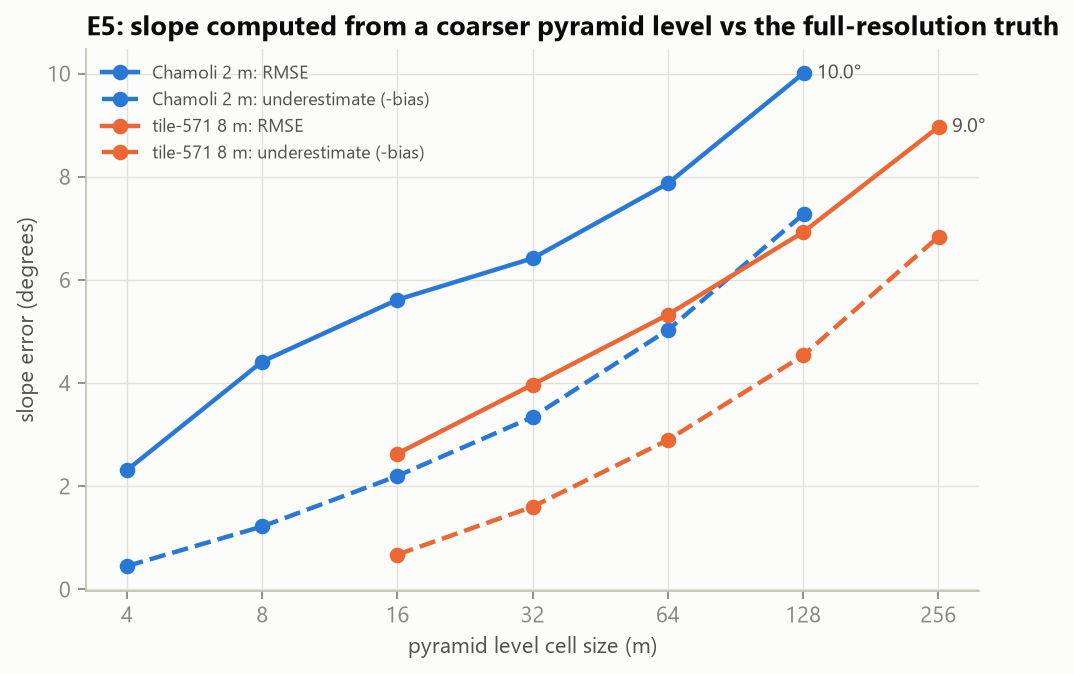
\includegraphics[width=0.49\linewidth]{e5_error_by_level.png}\hfill
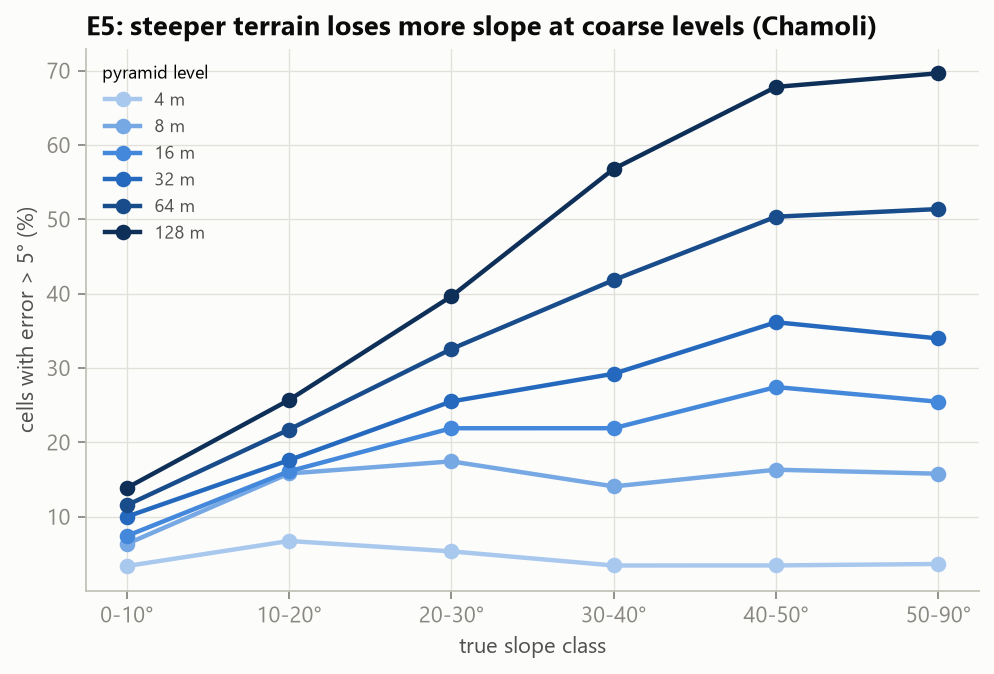
\includegraphics[width=0.49\linewidth]{e5_by_class.png}
\caption{Left: slope RMSE and underestimate ($-$bias) per pyramid level for both DEMs. Right: share of cells off
by more than 5$^\circ$ by true-slope class (Chamoli): steep terrain loses the most.}
\label{fig:err}
\end{figure}

\begin{itemize}
  \item \textbf{Slope from a coarse level is too low, and more so the coarser the level.} Averaging the DEM smooths
  the terrain before slope is computed, which removes steepness; the mean slope shown drops from 99\% to 81\% of the
  true mean on Chamoli. This agrees with the long-known decrease of computed slope with grid size
  \cite{zhang}; what is new here is the measurement on pyramid levels against the time saved.
  \item \textbf{What matters is how many levels up, not the cell size in metres.} The two DEMs give similar errors
  for the same number of levels up (within 0.5$^\circ$ up to four levels): about 2.5$^\circ$ RMSE one level up, then on
  average about 1.5$^\circ$ more per further level.
  \item \textbf{GDAL's overviews behave like an exact pyramid}: within 0.2$^\circ$ RMSE at every level, although
  their cells are not exactly $2^k$ fine cells. A viewer can use COG overviews as they are.
\end{itemize}

\begin{figure}[!htbp]
\centering
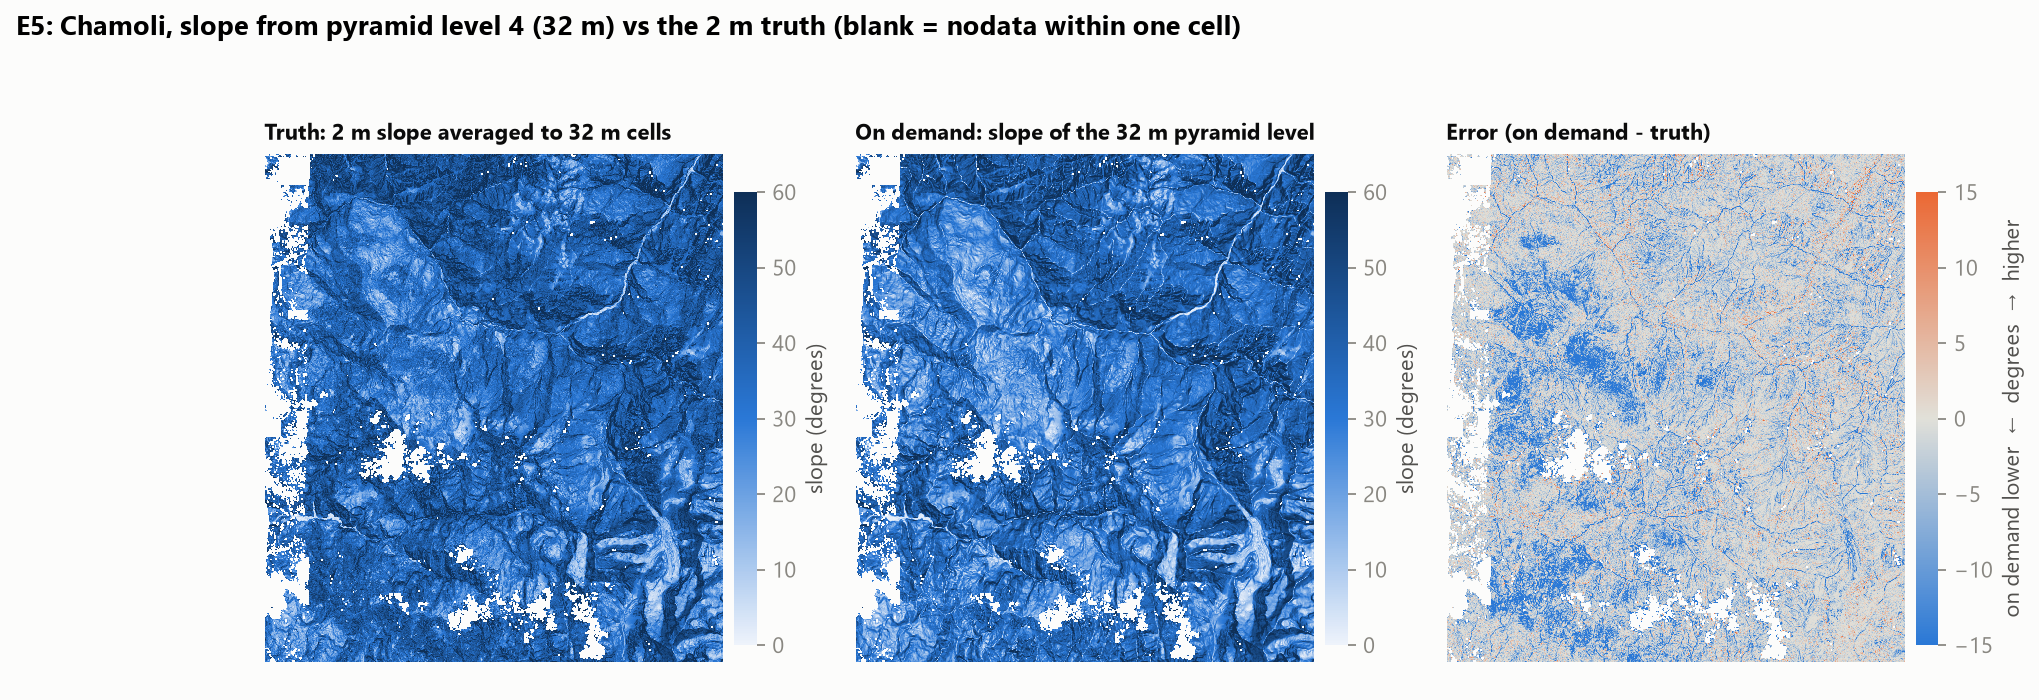
\includegraphics[width=\linewidth]{e5_maps.png}
\caption{Chamoli at 32\,m. Left: truth (2\,m slope averaged to 32\,m cells). Middle: slope computed on demand from
the 32\,m pyramid level. Right: error; blue = on demand lower. The on-demand map keeps every valley, ridge and
landslide scar but is lower almost everywhere, most on rough, broken slopes.}
\label{fig:maps}
\end{figure}

\subsection{Steep terrain and slope thresholds}

\begin{table}[!htbp]
\centering\small
\caption{Chamoli: bias by true-slope class, and the share of cells at or above 45$^\circ$ in truth and on demand.}
\label{tab:class}
\begin{tabularx}{\linewidth}{lRRRRRRRR}
\toprule
Level & 0--10$^\circ$ & 10--20$^\circ$ & 20--30$^\circ$ & 30--40$^\circ$ & 40--50$^\circ$ & 50--90$^\circ$ &
$\geq$45$^\circ$ truth & $\geq$45$^\circ$ shown \\
\midrule
4\,m & $-$0.1 & $-$0.2 & $-$0.3 & $-$0.3 & $-$0.6 & $-$0.8 & 33.2\% & 32.1\% \\
8\,m & $-$0.0 & $-$0.2 & $-$0.7 & $-$1.0 & $-$1.6 & $-$2.0 & 32.3\% & 29.2\% \\
16\,m & $-$0.5 & $-$0.8 & $-$1.4 & $-$2.0 & $-$2.8 & $-$3.0 & 30.8\% & 25.7\% \\
32\,m & $-$0.9 & $-$1.5 & $-$2.6 & $-$3.3 & $-$4.0 & $-$3.9 & 29.3\% & 21.9\% \\
64\,m & $-$0.7 & $-$1.9 & $-$3.5 & $-$5.1 & $-$6.0 & $-$5.9 & 28.4\% & 16.5\% \\
128\,m & $-$0.8 & $-$2.4 & $-$4.3 & $-$7.3 & $-$8.8 & $-$8.9 & 27.4\% & \textbf{10.1\%} \\
\bottomrule
\end{tabularx}
\end{table}

Steep cells lose the most: at 32\,m the bias is $-$0.9$^\circ$ on 0--10$^\circ$ ground but $-$4.0$^\circ$ on
40--50$^\circ$ ground, and 36\% of the 40--50$^\circ$ cells are off by more than 5$^\circ$ (10\% on flat ground).
Many uses of slope are a threshold (landslide susceptibility, ``too steep to build''). One level up, a threshold
map at 30$^\circ$ or 45$^\circ$ still agrees on 97\% of cells; four levels up a quarter of the terrain steeper than
45$^\circ$ has disappeared, and six levels up almost two thirds.

\subsection{Aspect}
The direction a slope faces is set by large landforms and survives smoothing. On Chamoli the median aspect error is
1.8$^\circ$ at 4\,m, 3.8$^\circ$ at 8\,m, 6.3$^\circ$ at 32\,m and 8.5$^\circ$ at 128\,m; only 1.4\% (4\,m) to
13.7\% (128\,m) of cells are off by more than 22.5$^\circ$, the width of one 16-point compass sector. The 8\,m DEM
gives the same picture (median 2.8$^\circ$ at 16\,m to 9.9$^\circ$ at 256\,m).

\subsection{Pyramid error vs differences between data sources}

\begin{figure}[!htbp]
\centering
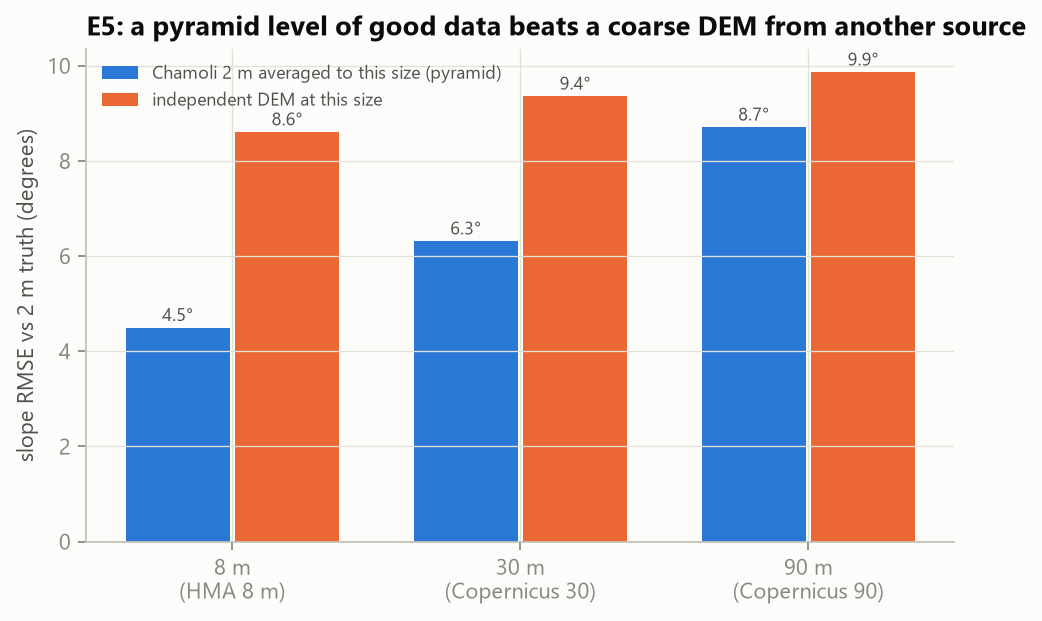
\includegraphics[width=0.62\linewidth]{e5_sensors.png}
\caption{Slope RMSE against the 2\,m truth over the Chamoli footprint: the 2\,m data averaged to 8, 30 and 90\,m
(a pyramid level) vs an independent DEM at the same resolution.}
\label{fig:sensors}
\end{figure}

At every resolution the pyramid of the 2\,m data is closer to the truth than a DEM measured natively at that
resolution by another sensor: 4.5$^\circ$ vs 8.6$^\circ$ for HMA 8\,m, 6.3$^\circ$ vs 9.4$^\circ$ for Copernicus
30\,m, 8.7$^\circ$ vs 9.9$^\circ$ for Copernicus 90\,m (Figure~\ref{fig:sensors}). At 8\,m the difference between the
two sources (7.3$^\circ$ RMSE) is larger than what the pyramid loses; at 90\,m the sources agree well (3.3$^\circ$) and
most of the error of both is simply the coarse resolution. When a high-resolution DEM exists, its pyramid is the
better coarse product.

\subsection{Time per view}

\begin{table}[!htbp]
\centering\small
\caption{One $512\times512$ display tile, median of 8 places (ms, warm / cold), and the time saved by computing on
demand instead of from full resolution (warm).}
\label{tab:time}
\begin{tabularx}{\linewidth}{llRRRR}
\toprule
DEM & Level & On demand & Full resolution + average & Precomputed & Time saved \\
\midrule
Chamoli & 2\,m (level 0) & 5.2 / 6.7 & = on demand & 4.1 / 5.2 & -- \\
 & 4\,m & 7.2 / 7.6 & 56 / 55 & 5.0 / 6.1 & \textbf{7.8$\times$} \\
 & 8\,m & 6.4 / 7.3 & 192 / 194 & 4.3 / 5.3 & \textbf{30$\times$} \\
 & 16\,m & 6.6 / 7.3 & 624 / 626 & 3.8 / 4.9 & \textbf{94$\times$} \\
 & 32\,m & 6.4 / 6.8 & 2867 / 2823 & 3.8 / 4.8 & \textbf{447$\times$} \\
\midrule
HMA 8\,m & 16\,m & 6.9 / 7.1 & 52 / 57 & 4.2 / 5.3 & 7.6$\times$ \\
 & 32\,m & 7.2 / 7.5 & 186 / 192 & 4.5 / 6.2 & 26$\times$ \\
 & 64\,m & 7.1 / 7.6 & 380 / 400 & 4.1 / 5.3 & 54$\times$ \\
 & 128\,m & 6.2 / 7.0 & 1186 / 1204 & 3.2 / 4.1 & 193$\times$ \\
\bottomrule
\end{tabularx}
\end{table}

\begin{figure}[!htbp]
\centering
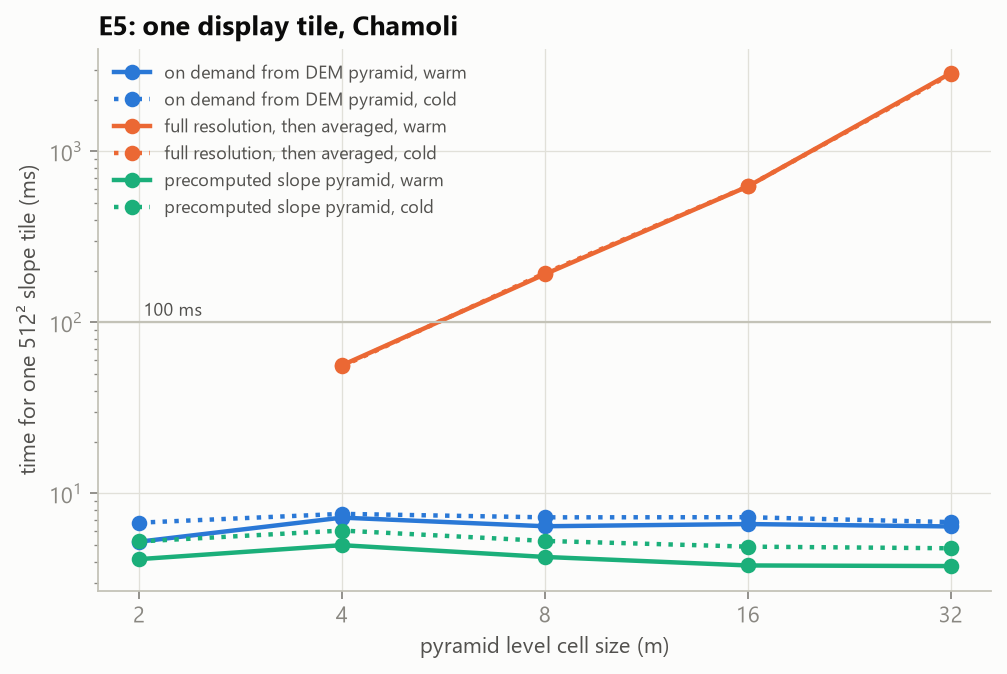
\includegraphics[width=0.49\linewidth]{e5_tile_time.png}\hfill
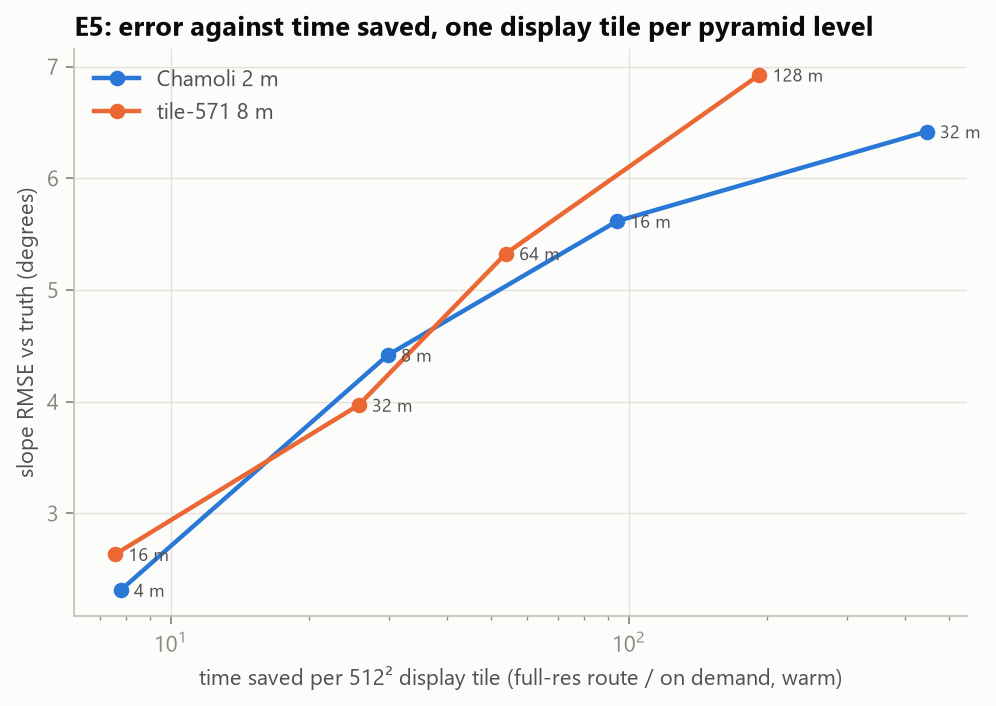
\includegraphics[width=0.49\linewidth]{e5_tradeoff.png}
\caption{Left: time for one display tile per pyramid level (Chamoli), three routes, cold and warm. Right: the G2
trade-off: slope RMSE against the time saved per tile, one point per pyramid level.}
\label{fig:time}
\end{figure}

\begin{itemize}
  \item \textbf{On demand costs the same at every zoom level} (5--8\,ms per tile): a tile always means reading
  $514^2$ cells and running the kernel on them. The exact full-resolution route reads 4$\times$ more ground per level
  and grows 2--5$\times$ per level, to 2.9\,s for one tile at 32\,m. For the whole Chamoli area at 32\,m, on demand
  takes 13\,ms against 4.7\,s.
  \item \textbf{Cold vs warm hardly matters} on this NVMe SSD: at most 1.5\,ms per tile for on demand.
  \item \textbf{Precomputed is about 1--3\,ms faster per tile} (it skips the slope kernel, about 0.5\,ms, and the
  window preparation). On demand and precomputed both stay far below the $\sim$100\,ms at which an interaction
  starts to feel slow; the full-resolution route exceeds it from two levels up.
\end{itemize}

\paragraph{The cost of precomputing.} A slope pyramid built in advance is exact and slightly faster per tile, but it
costs a full pass for every derivative: for Chamoli 10.6\,s (1.6\,s slope, 9.0\,s compression and overviews) and
1.0\,GB, more than the DEM pyramid itself (650\,MB), because slope compresses worse than elevation. The ten
\texttt{gdaldem} configurations would need about 10\,GB, rebuilt whenever a parameter (sun angle, z-factor, method) or
the DEM changes. On demand needs none of it.

\section{Discussion}
\paragraph{The G2 trade-off.} Each pyramid level up saves 2--5$\times$ in time per view (8--450$\times$ per tile for
one to four levels on Chamoli, 8--190$\times$ on the 8\,m DEM) and costs about 2.5$^\circ$ slope RMSE for the first
level and about 1.5$^\circ$ more per further level on average, as a systematic underestimate that is largest on
steep ground. Aspect costs much less (median 2--8$^\circ$).

\paragraph{Implications for the interactive viewer (Phase 5).}
\begin{itemize}
  \item Choose the pyramid level so that one level cell is about one screen pixel: the on-demand value is then
  close to what that pixel should show, and every tile costs 5--8\,ms, of which about 0.5\,ms is the slope kernel.
  \item Precompute only the one or two most used products (slope), if storage allows; compute everything else on
  demand, including any hillshade sun angle.
  \item Add a decoded-tile cache: re-reading compressed blocks, not the kernel, is the main cost of a tile.
  \item For analysis rather than display, never threshold slope computed from a coarse level: compute the view at full
  resolution (0.05--2.9\,s per tile here) or read a precomputed slope pyramid.
\end{itemize}

\paragraph{Limitations.} One region of steep terrain (mean true slope 38$^\circ$ on Chamoli, 31$^\circ$ on the 8\,m
area); flatter regions would show smaller errors, and the per-class tables carry over. The truth is itself a DEM
with its own noise, and the 8\,m DEM's truth is only 8\,m. The fully-valid rule scores fewer cells at coarse
levels (17\% of cells at 256\,m on the 8\,m DEM, whose data gaps lie in steep terrain). Timing is on one machine with
a local NVMe SSD; a network-hosted COG would add latency per request and widen the gap between the routes. The
underestimate is systematic, so a per-level correction factor could remove most of the bias, but not the spread;
this was not tested.

\section{Next step}
\textbf{Box-zoom viewer (E6).} Instead of streaming pyramid tiles while the user pans and scrolls, the viewer shows
the whole map and lets the user drag a box on it; only that box is computed (slope, aspect or hillshade) at the
pyramid level where one cell is about one screen pixel, with the expected error from this report shown next to it,
or exactly from full resolution on request. A second box inside the view zooms deeper, and so on down to full
resolution. A web viewer and a QGIS plugin will share one server, and E6 will measure the time per zoom step by stage
(read, compute, colour map, display), CPU vs GPU, at every zoom depth.

\begin{thebibliography}{9}\small
\bibitem{chamoli} Bhushan, S., \& Shean, D. (2021). Chamoli Disaster Pre-event 2-m DEM Composite: September 2015.
Zenodo. doi:10.5281/zenodo.4554647.
\bibitem{hma8} Shean, D. (2017). High Mountain Asia 8-meter DEM Mosaics Derived from Optical Imagery, Version 1.
NASA NSIDC DAAC. doi:10.5067/KXOVQ9L172S2.
\bibitem{cop30} European Space Agency (2021). Copernicus Global Digital Elevation Model (GLO-30). Distributed by
OpenTopography. doi:10.5069/G9028PQB.
\bibitem{horn} Horn, B.\,K.\,P. (1981). Hill shading and the reflectance map. \emph{Proceedings of the IEEE},
69(1), 14--47.
\bibitem{zhang} Zhang, W., \& Montgomery, D.\,R. (1994). Digital elevation model grid size, landscape
representation, and hydrologic simulations. \emph{Water Resources Research}, 30(4), 1019--1028.
\end{thebibliography}

\end{document}
